
    \begin{figure}[!hp]
	\centering
	\resizebox{\columnwidth}{!}{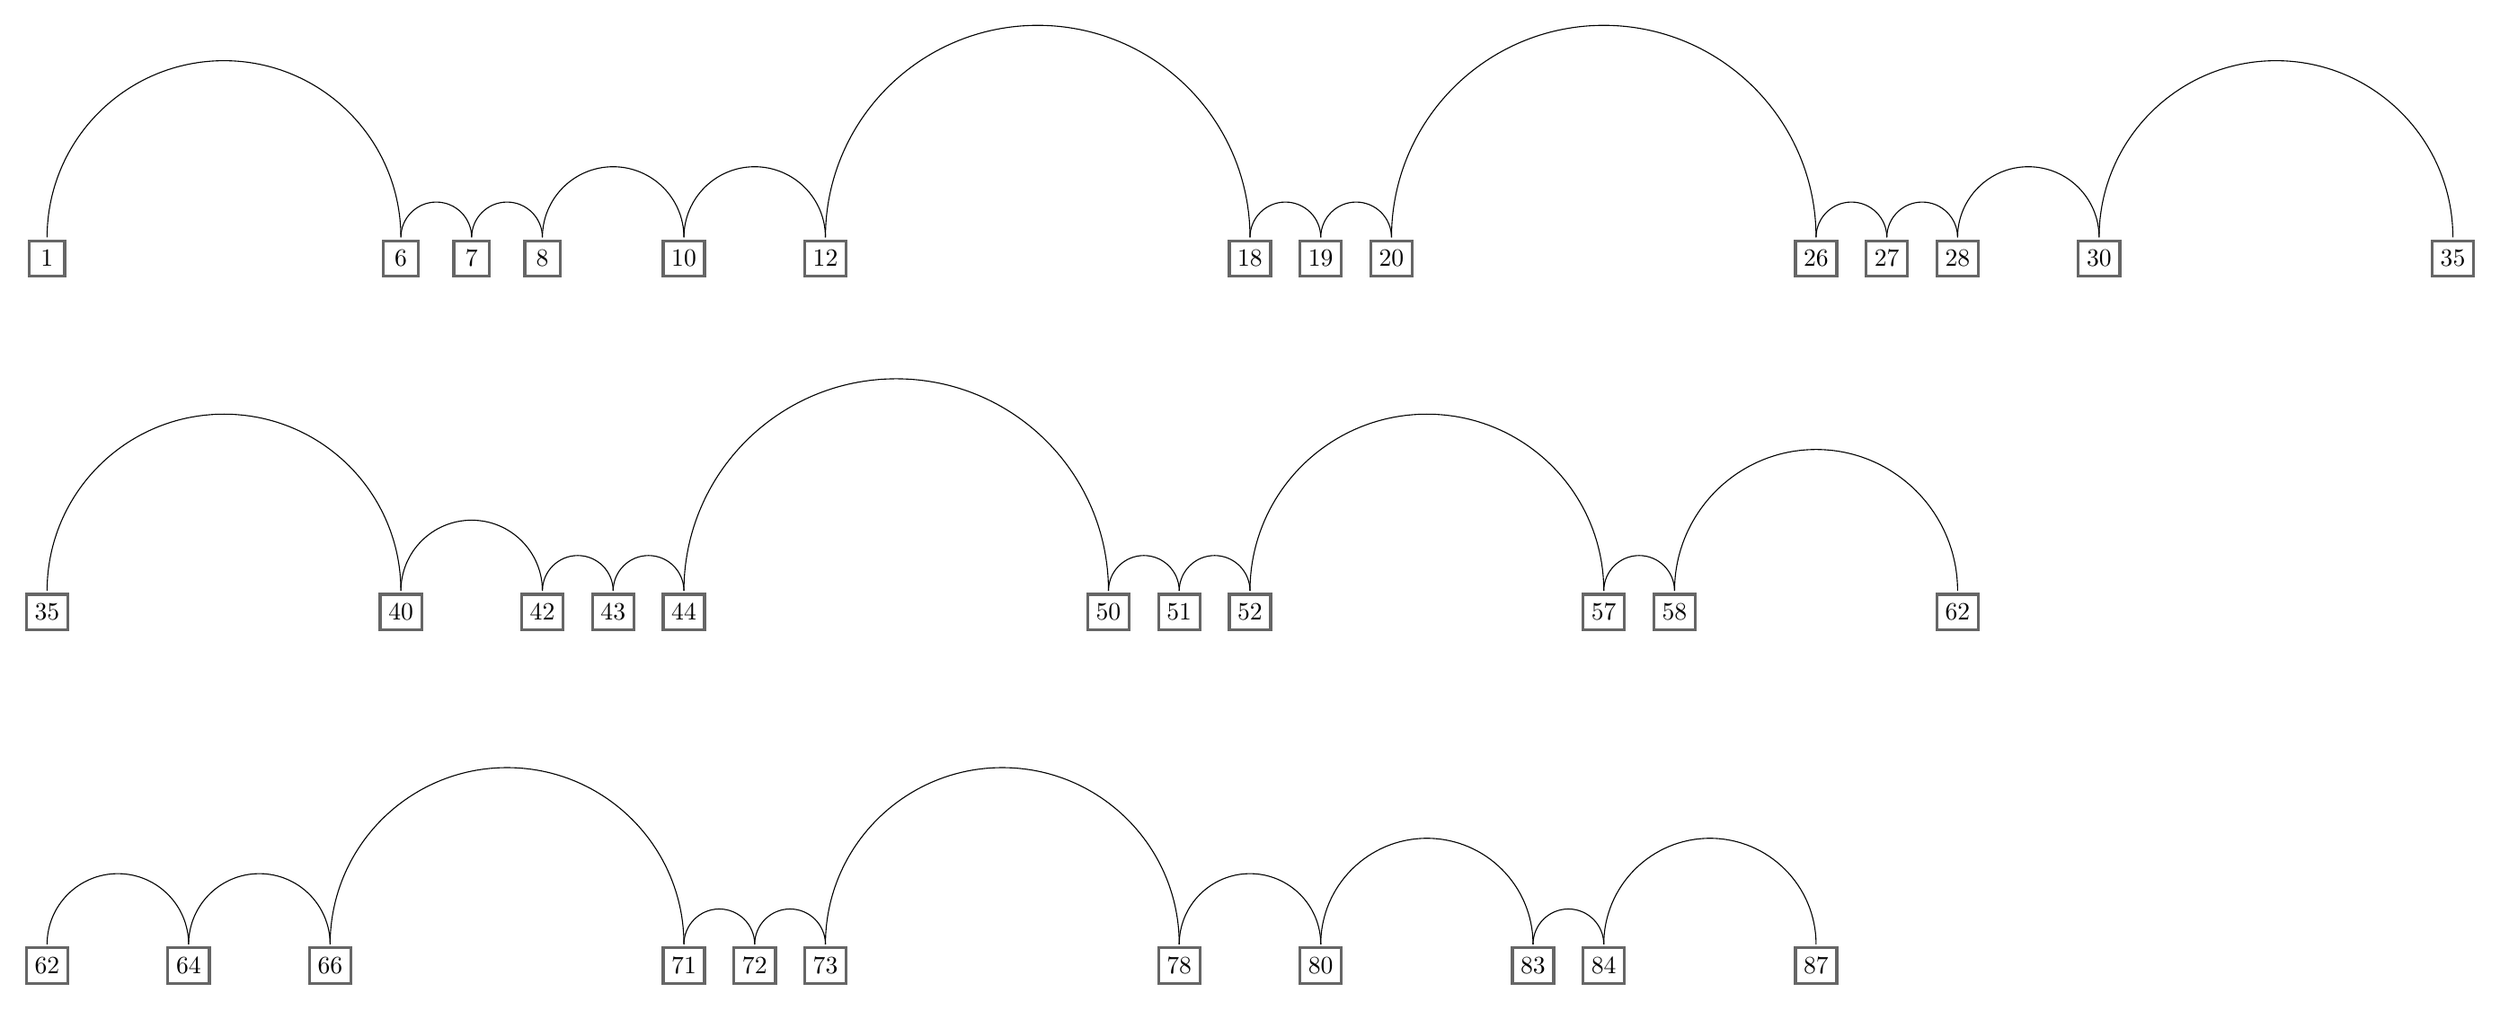
\begin{tikzpicture}[
			squareblack/.style={rectangle, draw=black!60, fill=white!5, very thick, minimum size=5mm},
			]
			\centering


    \node[squareblack] (1000) at (0.0,0) {1};
\node[squareblack] (6000) at (5.0,0) {6};
\draw[black] (6000)+(0,0.3) arc (0:180:2.5);
\node[squareblack] (7000) at (6.0,0) {7};
\draw[black] (7000)+(0,0.3) arc (0:180:0.5);
\node[squareblack] (8000) at (7.0,0) {8};
\draw[black] (8000)+(0,0.3) arc (0:180:0.5);
\node[squareblack] (10000) at (9.0,0) {10};
\draw[black] (10000)+(0,0.3) arc (0:180:1.0);
\node[squareblack] (12000) at (11.0,0) {12};
\draw[black] (12000)+(0,0.3) arc (0:180:1.0);
\node[squareblack] (18000) at (17.0,0) {18};
\draw[black] (18000)+(0,0.3) arc (0:180:3.0);
\node[squareblack] (19000) at (18.0,0) {19};
\draw[black] (19000)+(0,0.3) arc (0:180:0.5);
\node[squareblack] (20000) at (19.0,0) {20};
\draw[black] (20000)+(0,0.3) arc (0:180:0.5);
\node[squareblack] (26000) at (25.0,0) {26};
\draw[black] (26000)+(0,0.3) arc (0:180:3.0);
\node[squareblack] (27000) at (26.0,0) {27};
\draw[black] (27000)+(0,0.3) arc (0:180:0.5);
\node[squareblack] (28000) at (27.0,0) {28};
\draw[black] (28000)+(0,0.3) arc (0:180:0.5);
\node[squareblack] (30000) at (29.0,0) {30};
\draw[black] (30000)+(0,0.3) arc (0:180:1.0);
\node[squareblack] (35000) at (34.0,0) {35};
\draw[black] (35000)+(0,0.3) arc (0:180:2.5);\node[squareblack] (35000) at (0.0,-5) {35};
\node[squareblack] (40000) at (5.0,-5) {40};
\draw[black] (40000)+(0,0.3) arc (0:180:2.5);
\node[squareblack] (42000) at (7.0,-5) {42};
\draw[black] (42000)+(0,0.3) arc (0:180:1.0);
\node[squareblack] (43000) at (8.0,-5) {43};
\draw[black] (43000)+(0,0.3) arc (0:180:0.5);
\node[squareblack] (44000) at (9.0,-5) {44};
\draw[black] (44000)+(0,0.3) arc (0:180:0.5);
\node[squareblack] (50000) at (15.0,-5) {50};
\draw[black] (50000)+(0,0.3) arc (0:180:3.0);
\node[squareblack] (51000) at (16.0,-5) {51};
\draw[black] (51000)+(0,0.3) arc (0:180:0.5);
\node[squareblack] (52000) at (17.0,-5) {52};
\draw[black] (52000)+(0,0.3) arc (0:180:0.5);
\node[squareblack] (57000) at (22.0,-5) {57};
\draw[black] (57000)+(0,0.3) arc (0:180:2.5);
\node[squareblack] (58000) at (23.0,-5) {58};
\draw[black] (58000)+(0,0.3) arc (0:180:0.5);
\node[squareblack] (62000) at (27.0,-5) {62};
\draw[black] (62000)+(0,0.3) arc (0:180:2.0);\node[squareblack] (62000) at (0.0,-10) {62};
\node[squareblack] (64000) at (2.0,-10) {64};
\draw[black] (64000)+(0,0.3) arc (0:180:1.0);
\node[squareblack] (66000) at (4.0,-10) {66};
\draw[black] (66000)+(0,0.3) arc (0:180:1.0);
\node[squareblack] (71000) at (9.0,-10) {71};
\draw[black] (71000)+(0,0.3) arc (0:180:2.5);
\node[squareblack] (72000) at (10.0,-10) {72};
\draw[black] (72000)+(0,0.3) arc (0:180:0.5);
\node[squareblack] (73000) at (11.0,-10) {73};
\draw[black] (73000)+(0,0.3) arc (0:180:0.5);
\node[squareblack] (78000) at (16.0,-10) {78};
\draw[black] (78000)+(0,0.3) arc (0:180:2.5);
\node[squareblack] (80000) at (18.0,-10) {80};
\draw[black] (80000)+(0,0.3) arc (0:180:1.0);
\node[squareblack] (83000) at (21.0,-10) {83};
\draw[black] (83000)+(0,0.3) arc (0:180:1.5);
\node[squareblack] (84000) at (22.0,-10) {84};
\draw[black] (84000)+(0,0.3) arc (0:180:0.5);
\node[squareblack] (87000) at (25.0,-10) {87};
\draw[black] (87000)+(0,0.3) arc (0:180:1.5);

        \end{tikzpicture}}
    \end{figure}
